\documentclass{beamer}
%\AtBeginDvi{\special{pdf:tounicode 90ms-RKSJ-UCS2}}
\usetheme{Madrid}
\usepackage{multirow}
\usepackage{alltt}
\usepackage{hyperref}

\usepackage{tikz}
\usetikzlibrary{arrows,calc}
\tikzstyle{block}=[draw opacity=0.7,line width=1.4cm]


\title[ISAT-based Method with Native BC for HCP]{%
Incremental SAT-based Method with \\ Native Boolean Cardinality Handling for\\ the Hamiltonian Cycle Problem}
\author[\tiny{Soh {\it et al.}}]{
  Takehide Soh\inst{1} \and 
  Daniel Le Berre\inst{2} \and 
  St\'{e}phanie Roussel\inst{2} \and \\
  Naoyuki Tamura\inst{1} \and 
  Mutsunori Banbara\inst{1}}
\institute[Kobe University]{
  \inst{1} 
 Information Science and Technology Center, Kobe University \and 
  \inst{2} 
CRIL-CNRS, UMR 8188, Universit\'e d'Artois
  }
\date{2014/07/11 @ University of Potsdam}

\setbeamertemplate{navigation symbols}{}
\setbeamertemplate{footline}[page number]

\newcommand{\vr}{\vrule}
\newcommand{\en}{\vrule depth 0.4pt \vrule height 0em width 0.5em
depth 0.4pt}

\newcommand{\cen}[2]{\multicolumn{#1}{c}{#2}}
\newcommand{\mul}[2]{\multirow{#1}{*}{#2}}

\begin{document}
\frame{\titlepage}

%-----------------------------------------
% page
%-----------------------------------------
\begin{frame}{Self-Introduction}
\begin{columns}
\begin{column}{0.5\textwidth}
\begin{center}
\includegraphics[width=\textwidth]{figs/career0.eps}<1>
\includegraphics[width=\textwidth]{figs/career.eps}<2->
\end{center}
\end{column}
\begin{column}{0.5\textwidth}
\begin{enumerate}
\item 2011.10\\ got Ph.D., in Inoue Lab, NII.\\
SAT-based Problem Solving\\
Scheduling, Packing, Biological Problem.
\item (Current)\\ Tamura Lab., Kobe Univ. \\
working with Prof. Tamura and Prof. Banbara.
%\item<3> 2014.11 get married!
\end{enumerate}
\end{column}
\end{columns}

% \begin{columns}
% \begin{column}{0.3\textwidth}
% \begin{center}
% \includegraphics[width=\textwidth]{figs/career.eps}\\
% Takehide SOH
% \end{center}
% \end{column}
% \begin{column}{0.7\textwidth}
% \begin{enumerate}
% \item 2011.10\\ got Ph.D., in Inoue Lab, National Institute of Informatics.\\
% SAT-based approach for solving 2SPP and analizing metabolic pathway. 
% \item Current\\ Kobe Univ., working with Prof. Tamura and Prof. Banbara.
% \end{enumerate}
% \end{column}
% \end{columns}
    % \centering
    % \includegraphics[width=\hsize]{./figs/career.eps}
\end{frame}

\begin{frame}{Problem Solving using ASP, PB, SMT, SAT etc. Solver}
  \centering
  \includegraphics[width=0.8\hsize]{./figs/cspsat.eps}
    \begin{itemize}
    \item Problem solving is usually processed by a-b-c-d-e.
    \item Many research topics in this field. Among them, the
      importance of modeling and encoding are re-recognized (Invited
      Talk by Prof. Stuckey, SAT 2013). 
    \item Good modeling/encodings are developed considering the size of
      solver input and propagation in solvers (and many many
      trial/errors are necessary!). However, sometimes there is no way
      but to generate extremely large solver input. 
    \end{itemize}
 \pause
     \begin{block}{}
       We show one way of escaping this limitation using HCP as an instance.
     \end{block}
\end{frame}

\begin{frame}{Hamiltonian cycle problem}
\begin{center}
\begin{minipage}[c]{0.3\textwidth}
  \begin{figure}
    \centering
    \includegraphics[width=0.9\hsize]{./figs/hcpcsp_undirected.eps}<1>
  \end{figure}
\end{minipage}  
\begin{minipage}[c]{0.3\textwidth}
  \begin{figure}
    \centering
    \includegraphics[width=0.9\hsize]{./figs/hcpcsp_undirected_cycle.eps}<1>
  \end{figure}
\end{minipage}  
\end{center}  

\begin{itemize}
\item The \structure{Hamiltonian cycle problem} (HCP) is an NP-complete problem of 
finding a spanning cycle, called \structure{Hamiltonian cycle}, in a given graph.
\item HCP is NP-complete and has been known as an important problem due to
its close relation to the travelling salesman problem (TSP). 
\item TSP can be seen as an optimization variant of HCP and the development
of an effective method for TSP would have a significant impact in
computer science. 
\end{itemize}
\end{frame}

\begin{frame}{Constraint Model of HCP: Constraints}% (by [Dantzig '54])}
$V$ is a set of $n$ \structure{nodes}, $A$ is a set of \structure{arcs}, and $G = (V, A)$ is a
\structure{digraph}. \\
\centering{$x_{ij} = 1 \Leftrightarrow \text{$(i,j) \in A$ is used in a solution cycle}$}

\begin{block}{}
\vspace{-1em}
\begin{align}
%minimize \quad& \sum c_{ij} x_{ij}&\\
&\sum_{(i,j) \in A} x_{ij}=1 & ~\text{for each}~ i=1,\ldots,n\notag
 ~~\text{(out-degree)}\\
&\sum_{(i,j) \in A}^{n} x_{ij}=1 & ~\text{for each}~ j=1,\ldots,n\notag
~~\text{(in-degree)}\\
&\sum_{i,j \in S} x_{ij} \le |S| - 1 & S \subset V,~ 2\le |S| \le
n-2 \notag ~~\text{(connectivity)}
\end{align}
\end{block}
\begin{itemize}
\item \structure{in/out-degree constraints} ensure that in-degree and
  out-degree are respectively exact one for each node in solution cycles. 
\item \structure{connectivity constraint} prohibits the formulation of sub-cycles, i.e.,
  cycles on subsets of less than $n$ nodes ($x_{ij} + x_{ji} \le 1$ is also included).
\end{itemize}
\end{frame}

\begin{frame}{Role of Each Constraint}
\begin{itemize}
\item With only in/out-degree constraints, we have cycles but they may not connected (Case A). 
\item With all constraints, we can find a Hamiltonian cycle (Case B).
\end{itemize}

\begin{center}
\begin{minipage}[c]{0.45\textwidth}
  \begin{figure}
    \centering
    \includegraphics[width=0.8\hsize]{./figs/hcpcsp_cycles.eps}
  \end{figure}
\vspace{-1em}
  \centering
(Case A)\\
in/out-degree
\end{minipage}
\begin{minipage}[c]{0.45\textwidth}
  \begin{figure}
    \centering
    \includegraphics[width=0.8\hsize]{./figs/hcpcsp_spanningcycles.eps}
  \end{figure}
\vspace{-1em}
  \centering
(Case B)\\
in/out-degree $+$ connectivity
\end{minipage}
\end{center}
\end{frame}

\begin{frame}{SAT-based Methods for HCP}
\begin{block}{Previous Methods until 2003}
\begin{itemize}
\item \mbox{}\structure{{\bf \cite{DBLP:conf/ifip/IwamaM94}}} log encoding
\item \mbox{}\structure{{\bf \cite{DBLP:conf/ijcai/Hoos99}}} absolute encoding
\item \mbox{}\structure{{\bf \cite{DBLP:journals/dam/Prestwich03}}} relative encoding
\begin{itemize}
\item It encodes connectivity constraint using transitive relations for any
  three nodes, which results in \alert{{\bf $O(n^{3})$ clauses}}.
\end{itemize}
\end{itemize}
\end{block}

\pause
\begin{block}{\cite{DBLP:conf/ausai/VelevG09}}
\begin{itemize}
\item \mbox{}\structure{Velev and Gao} basically follows
\cite{DBLP:journals/dam/Prestwich03}
 but they reduce encoded clauses by improving ordering variables and a triangulation for a given digraph. 
The improved method achieves 4 orders of magnitude speedup on structured instances.
\end{itemize}
\end{block}

\pause
\begin{alertblock}{}
However, it is hard to solve HCP of over 1000 nodes by SAT-based
methods while the state-of-the-art HCP/TSP solver \textsf{LKH} scales up to 10000 nodes. 
\end{alertblock}
\end{frame}

\begin{frame}{Main Ideas to Escape the Current Limitations.}
\begin{enumerate}
\item \structure{{\bf Incremental HCP Solving (CEGAR-HCP)}}
\begin{itemize}
\item No longer encode connectivity constraints but refine overall
  constraints by adding blocking clauses generated from counter examples.
\end{itemize}
\item \structure{{\bf Native Boolean Cardinality Handling}}
\begin{itemize}
\item in/out-degree constraints $\sum_{(i,j) \in A} x_{ij}=1$ can be
  represented in Boolean cardinality (BC) constraints.
\item Instead of encoding BC constraints, use the native BC handling function of SAT solvers.
\end{itemize}
\item \structure{{\bf Tight Integrated System with SAT Solvers}}
\begin{itemize}
\item SAT-based systems (e.g., Sugar) are loosely integrated
  with SAT solvers would cause communication overhead. 
%\item<4-> \alert{It is expected to reduce communication overhead.}<4->
\end{itemize}
\end{enumerate}
\begin{block}{}
\begin{itemize}
\item Ideas 1 and 2 are expected to reduce the number of SAT clauses encoded.
\item We also can save encoding time of BC.
\end{itemize}
\end{block}
\end{frame}

\begin{frame}{CEGAR-HCP}
\begin{block}{}%\mbox{\bf HCPのインクリメンタルSAT解法}~($G, G'$)}
\begin{figure}[t!]
\begin{tabbing}
\hspace{1.5em}\=\hspace{1em}\=\hspace{1em}\=\hspace{1em}\=\hspace{1em}\=\hspace{1em}\=\hspace{1em}\=\hspace{1em}\=\hspace{1em}\=\hspace{1em}\=\hspace{1em}\=\hspace{1em}\kill
%\> \mbox{\bf begin}\\ 
{\small 1:}\> $\Psi$ := Encode only in/out-degree constraints from $G$~;\\
{\small 2:}\> \mbox{\bf while}~({\sf SAT Solve}($\Psi$))\\
{\small 3:}\> \> \vr \> \mbox{\bf if} (Solution contains only one cycle)\\
{\small 4:}\> \> \vr \> \> \vr \> \structure{{\bf return} \structure{a
    spanning cycle of $G$}}; \\
{\small 5:}\> \> \vr \> \mbox{\bf else} \\
{\small 6:}\> \> \vr \> \> \en \> 
      $\Psi_{block}$ := Construct block clauses from multiple sub-cycles;\\
{\small 7:}\> \> \en \> $\Psi := \Psi \wedge \Psi_{block}$~;\\
{\small 8:}\> \structure{{\bf return} \structure{there is no spanning cycle}};
%\> \mbox{\bf end}
\end{tabbing}
\end{figure}
\end{block}
%\pause{}
\begin{minipage}[c]{0.4\textwidth}
  \begin{figure}
    \centering
    \includegraphics[width=0.8\hsize,clip]{./figs/hcpcsp_cycles_number.eps}
  \end{figure}  
\end{minipage}  
%\pause{}
\begin{minipage}[c]{0.55\textwidth}
\begin{block}{Blocking Clauses}
\structure{$C_1$} $\neg x_{12} \vee \neg x_{23} \vee \neg x_{37} \vee \neg x_{78}\vee \neg x_{81}$\\
\structure{$C_1'$} $\neg x_{87} \vee \neg x_{73} \vee \neg x_{32}\vee \neg  x_{21} \vee \neg x_{18}$\\
\structure{$C_2$} $\neg x_{46} \vee \neg x_{65} \vee \neg x_{54}$\\
\structure{$C_2'$} $\neg x_{45} \vee \neg x_{56} \vee \neg x_{64}$
\end{block}
\end{minipage}
\end{frame}

\begin{frame}{Remarks}
\begin{minipage}[c]{0.4\textwidth}
  \begin{figure}
    \centering
    \includegraphics[width=0.8\hsize,clip]{./figs/hcpcsp_cycles_number.eps}
  \end{figure}  
\end{minipage}  
\begin{minipage}[c]{0.55\textwidth}
\begin{block}{Blocking Clauses}
\structure{$C_1$} $\neg x_{12} \vee \neg x_{23} \vee \neg x_{37} \vee \neg x_{78}\vee \neg x_{81}$\\
\structure{$C_1'$} $\neg x_{87} \vee \neg x_{73} \vee \neg x_{32}\vee \neg  x_{21} \vee \neg x_{18}$\\
\structure{$C_2$} $\neg x_{46} \vee \neg x_{65} \vee \neg x_{54}$\\
\structure{$C_2'$} $\neg x_{45} \vee \neg x_{56} \vee \neg x_{64}$
\end{block}
\end{minipage}
\begin{itemize}
\item Due to in/out-degree constraints, every node must belong to
  some cycles.
\item Then, it is {\bf NOT} necessary to enumerate all sub-cycles in a given
  graph (e.g., 1-2-3-4-8 in the example).
\item By adding blocking clauses for each sub-cycles, all solutions
  including sub-cycles appeared before are eliminated. 
\end{itemize}
\end{frame}

\begin{frame}{Native Boolean Cardinality Handling}
  \begin{itemize}
  \item Using CEGAR-HCP, we only need to encode in/out-degree constrains, which can be represented in Boolean Cardinality.
\end{itemize}
  \begin{block}{}
\centering
\begin{align*}
\sum_{i=1}^{n}x_{i} \ge k
\end{align*}
where $n$ be \#variables, $x_{i}$ be Boolean variables, and $k$ be threshold degree.
  \end{block}
\begin{itemize}
  \item SAT encoding of BC constraints has been actively studied
  \end{itemize}
\begin{center}
\begin{tabular}{lcc}
\hline
Method & \#Clauses & Check \\\hline
 Binomial Encoding & $\binom{n}{k+1}$ & immediate\\
Totalizer~\cite{DBLP:journals/jsat/BailleuxBR06} & $O(n\cdot{k})$ & unit propagation\\
Seq. Counter~\cite{DBLP:conf/cp/Sinz05} & $O(n\cdot{k})$ & unit propagation\\
\hline
\end{tabular}
\end{center}

    % \begin{itemize}
    % \item Binomial Encoding ($\binom{n}{k}$ clauses needed)
    % \item Totalizer [Bailleux '06] ($O(n^2)$ clauses needed)
    % \item Sequential Counter [Sinz '05] ($O(n\cdot{k})$ clauses needed)
    % \end{itemize}
\begin{itemize}
  \item However, it still generates a number of clauses when graph size becomes large.
  \end{itemize}
\end{frame}

\begin{frame}{Native BC in Sat4j~\cite{leberre10}}
  \begin{itemize}
  \item The \textsf{Sat4j} library started in 2004 as an
implementation in Java of the original \textsf{Minisat} 
specification~\cite{DBLP:conf/sat/EenS03}. 
\item In contrast to \textsf{Minisat2.2}, and most SAT solvers, the underlying SAT solver is still designed to work with custom constraints, not just clauses.
  \end{itemize}

  \begin{block}{}
\vspace{-1.5em}
\centering
\begin{align*}
\sum_{i=1}^{n}x_{i} \ge k
\end{align*}
\vspace{-1.3em}
\begin{description}
\item[Propagation] When $n-k$ literals are assigned to be false, then it forces to assign remaining un-assigned variables to be true.
\item[Conflict Detection] Conflict is detected when $n-k+1$ literals are assigned to false, then it returns those $n-k+1$ literals as a reason of the conflict detected. 
\end{description}
\begin{center}
\begin{tabular}{lcc}
\hline
Method & \#Clauses & Check \\\hline
Native BC & $\binom{n}{k+1}$ (in worst case) & immediate\\
\hline
\end{tabular}
\end{center}

  \end{block}
\end{frame}

% \begin{frame}{Native Boolean Cardinality Handling}
% \begin{itemize}
% \item SAT encoding of BC constraints has been actively studied
% \begin{itemize}
% \item Binomial Encoding ($\binom{n}{k}$ clauses needed)
% \item Totalizer [Bailleux '06] ($O(n^2)$ clauses needed)
% \item Sequential Counter [Sinz '05] ($O(n\cdot{k})$ clauses needed)
% \end{itemize}
% \item In contrast to most of all SAT solvers, \structure{\textsf{Sat4j}} is
%   designed so that it can treat custom constraints, not just clauses. 
% \item Among them, it has the native support for
%   cardinality constraint (\structure{Native BC}).
% \end{itemize}
% \begin{block}{}
% \begin{itemize}
% \item It currently emulates a BC constraint 
% $\sum_{i=1}^{n}x_{i} \ge k$ where $x_{i} \in \{0, 1\}$ are Boolean variables, $n$ is an integer
% represents the number of variables, $k$ is an integer represents the
% degree (threshold) of the constraint.
% \item Such specific constraints generates clauses of size $n-k+1$ when
% it detects a conflict with the current assignment.
% \item One can consider that such constraint generates ``on demand'' 
% or lazily the clauses of the binomial encoding.
% \end{itemize}
% \end{block}
% \end{frame}

%-----------------------------------------
% page
%-----------------------------------------
\begin{frame}{Experiments}
We evaluate the effectiveness of (1) CEGAR-HCP, (2) Native BC, \\
(3) Implementation on Tightly Integrated System. \\
We also have (4) a comparison with other specialized methods. 

\begin{block}{Machine Spec and Benchmark}
\begin{itemize}
\item CPU: Intel Xeon 2.93GHz, Memory: 4GB, Time Limit: 500 sec.
\item \structure{color04} (119 instances, $\#$nodes: 11 to 10000), \\\structure{knight} (11 instances, 8x8 to 100x100), \structure{tsplib} (9 instances)
\end{itemize}
\end{block}

\begin{block}{Systems Compared}
  \begin{itemize}[<+->]
\item CEGAR-HCP (on \textsf{Scarab})\\ \structure{S4J-S} (Seq. Counter), \structure{S4J-N} (Native BC)
  \item Eager Method \structure{Velev} (Minisat2.2)
\item Specialized TSP Solver \structure{LKH}\\ 
  (It holds all world records of TSP in TSPLIB)
\item CEGAR-HCP (on loosely integrated system) \structure{S4J-S-Loose}
  \end{itemize}
\end{block}
\end{frame}

\begin{frame}{Cactus Plot (\#Solved--CPU Time)}
\begin{center}
  \includegraphics[width=0.9\hsize]{./figs/st.eps}<1>
  \includegraphics[width=0.9\hsize]{./figs/st-note.eps}<2>
\end{center}
\end{frame}

\begin{frame}{Comparisons on \#Clauses}
\begin{columns}
\begin{column}{0.5\textwidth}
\centering
\includegraphics[width=\hsize]{./figs/velev-seq-clauses.eps}\\
\scriptsize
Eager vs. Incremental (Idea 1)
\end{column}
\begin{column}{0.5\textwidth}
\centering
\includegraphics[width=\hsize]{./figs/seq-native-clauses.eps}\\
\scriptsize
Seq. Counter vs. Native BC (Idea 2)
\end{column}
\end{columns}
\end{frame}

\begin{frame}{\#Iterations and \#Clauses}
\begin{center}
\begin{tabular}{llrrr}
\hline
\multicolumn{2}{c}{Statistics} & S4J-T & S4J-S & S4J-N \\
\hline
\mul{3}{~Iterations} \ 
&~Median    & 10 & 10 & 7 \\
&~Average   & 32.1 & 60.0 & 37.9 \\
&~Maximum   & 510 & 3332 & 761\\
\hline
\mul{3}{~Cycles}
&~Median    & 60 & 48 & 20 \\
&~Average   & 314.0 & 311.8 & 310.5\\
&~Maximum \ & 6759 & 9188 & 7604\\
\hline
\end{tabular}
\end{center}
\begin{itemize}
\item As the median numbers show, \#iterations and \#cycles are not so
  high in usual. 
\item The number of blocking clauses, which are necessary for
  incremental SAT solving, is at most 20 thousands. 
\item SAT solvers are sometimes launched over thousands times. 
\end{itemize}
\end{frame}

% \begin{frame}{Other Evaluations}
% We additionally have the following supplemental evaluations:
%   \begin{itemize}
%   \item Literature-based Comparison with \cite{DBLP:journals/anor/EshraghFH11}
%   \item Comparisons on Random Instances
%   \end{itemize}
% \end{frame}

\begin{frame}{Literature-based Comparison with \cite{DBLP:journals/anor/EshraghFH11}}
\begin{itemize}
\item \mbox{} \cite{DBLP:journals/anor/EshraghFH11} shows a hybrid algorithm and a Mixed Integer Programming (MIP) model for HCP on undirected graphs. 
\item They carried experiments on knight's tour problems of 8x8,
  12x12, and 20x20, and TSPLIB problems of \texttt{alb1000} and \texttt{alb2000}.
\item We have a literature-based comparison with \cite{DBLP:journals/anor/EshraghFH11}. 
\end{itemize}

\begin{center}
\begin{tabular}{lrrrr} \hline
  \mul{2}{Name} & 
  \mul{2}{Nodes} & 
  \mul{2}{Edges} & 
  \cen{2}{CPU Time (sec.)}\\\cline{4-5}
&&& [Eshragh '11] &  \textsf{S4J-N}\\\hline
  knight 8x8 & 64 & 168  & 2        &  1.2 \\
  knight 12x12 & 144 & 440 & 5      &  1.7 \\
  knight 20x20 & 400 & 1368 & 1731  &  4.3 \\
  alb1000 & 1000 & 1998 & 1907      &  5.8 \\
  alb2000 & 2000 & 3996 & 165600    &  7.2 \\\hline
\end{tabular}
\end{center}
\end{frame}

\begin{frame}{Comparisons on Random Instances}
\begin{center}
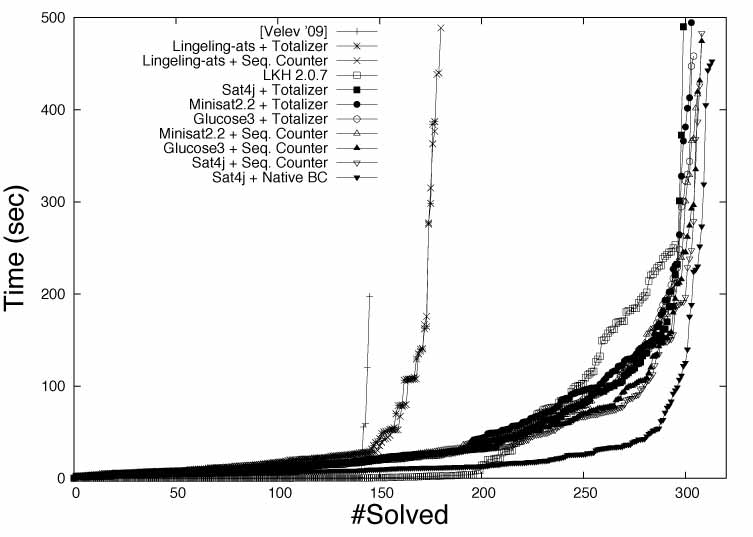
\includegraphics[width=0.8\hsize]{./figs/random.eps}
\end{center}
Our main 
motivation of using random instances is checking the scalability of 
the different approaches on different sizes on homogeneous graphs.
\end{frame}

\begin{frame}{Related Work}
  \begin{block}{CEGAR~\cite{DBLP:conf/cav/ClarkeGJLV00}}
    \begin{itemize}
    \item In 2000, Clarke \textit{et al.} proposed Counterexample-Guided
Abstraction Refinement (CEGAR) in the context of model
checking.
    \item It receives a program text and abstract functions are extracted from it
      \item CEGAR is well established in the context of model checking but
 there are not so many applications in other domains,
especially AI. 
    \end{itemize}    
  \end{block}

  \begin{block}{Studies in Operations Research}
    \begin{itemize}
    \item In the context of solving TSP, there is a traditional OR technique
proposed in 80's which translates TSP into an assignment
problem~\cite{capaneto80,TSP-AP-Laporte92}. 
    \item \cite{DBLP:journals/jair/JagerZ10}
applies this OR technique to HCP on directed graphs by using the
Hungarian algorithm and Karp-Steele patching. 
%
Though only for a small proportion of instances, a SAT approach is
used in their rare last step (14 out of 4266 instances) to guarantee
completeness.
    \end{itemize}
  \end{block}

\end{frame}

\begin{frame}{Conclusion}
\begin{itemize}
\item We proposed an incremental SAT-based method (CEGAR-HCP) with
  Native BC for solving HCP. 
\item CEGAR-HCP
\begin{itemize}
\item Constraints encoded are much (exponentially) reduced. 
\item It overcomes the eager method w.r.t. \#Solved instances. 
\end{itemize}
\item Native BC
\begin{itemize}
\item It has constant reduction of constrains compared to other BC
  encoding method Seq. counter and totalizer. 
\item It then improves the total cpu time. 
\end{itemize}
\item Implementation on tightly integrated systems
\begin{itemize}
\item In case of standard problem solving, loosely integrated systems
  can use any state-of-the-art SAT solvers without
  modifications. Also, the overhead of invoking SAT solvers is
  negligible. 
\item However, since \#iterations is sometimes almost 10 thousands,
  that cost affects to the performance in CEGAR. 
\end{itemize}
\end{itemize}

\pause
\begin{alertblock}{}
  \begin{itemize}[<+->]
    \item What is the appropriate system for this approach? \textbf{\alert{ASP!!}}
    \item Yes, we agree but let us explain our tool Scarab today :)
  \end{itemize}
\end{alertblock}
\end{frame}

\begin{frame}{Problem Solving using ASP, PB, SMT, SAT etc. Solver}
  \centering
  \includegraphics[width=0.8\hsize]{./figs/cspsat.eps}
    \begin{itemize}[<+->]
    \item CEGAR is processed by a-b-c-d-c-d-...-c-d-e.\\
      \alert{tight integration with solvers}.
    \item User may need many trial/errors to develop good constraint model.\\
      \alert{concise representation}.
    \item User may want customize encoder and native constraints.\\
      \alert{customizability}.
    \item \alert{Performance}. 
    \item \alert{Portability}. 
    \end{itemize}
 % \pause
 %     \begin{block}{}
 %       We show one way of escaping this limitation using HCP as an instance.
 %     \end{block}
\end{frame}

\begin{frame}{Tight Integrated System with SAT Solvers}
\begin{itemize}
\item \structure{\textsf{Scarab}} is a prototyping tool for developing SAT-based Constraint Programming (CP) systems.
\item <2-> It consists of 1) CP Domain-Specific Language, 2) API of CSP solver, 3) SAT encoding module, and 4) API of SAT solvers.
\item <2-> It uses \structure{Order Encoding} and \structure{Sat4j} in default.
\end{itemize}
    \centering
\only<1>{\includegraphics[width=\textwidth]{./figs/process_flow_v6-non.eps}}
%\only<2>{\includegraphics[width=\textwidth]{./figs/process_flow_v6-0.eps}}
\only<2>{\includegraphics[width=\textwidth]{./figs/process_flow_v6-01.eps}}
\only<3>{\includegraphics[width=\textwidth]{./figs/process_flow_v6-1.eps}}
\only<4>{\includegraphics[width=\textwidth]{./figs/process_flow_v6-2.eps}}
\only<5>{\includegraphics[width=\textwidth]{./figs/process_flow_v6-3.eps}}
\only<6->{\includegraphics[width=\textwidth]{./figs/process_flow_v6.eps}}

\begin{itemize}
\item<7-> It is developed to be an expressive, efficient, customizable, and portable workbench.
%\item<7-> It is developed to help users' to focus on problem modeling and encoding.
\item<8-> The tight integration to \textsf{Sat4j} enables advanced CSP
  solving such as incremental solving and the use of native constraints. 
\end{itemize}
\end{frame}

\begin{frame}{Feature of Scarab}
  \begin{itemize}
  \item Incremental SAT solving with assumption.
  \item Customizability of Encoders.
  \item Customizability of Native Constraints.
  \item Performance.
  \end{itemize}
\end{frame}

\begin{frame}{Comparisons with Loosely Integrated Systems using other SAT Solvers}
\begin{center}
\includegraphics[width=0.8\hsize]{./figs/all.eps}
\end{center}
\end{frame}

\begin{frame}{Feature of Scarab}
  \begin{itemize}
  \item Incremental SAT solving with assumption.
  \item Customizability of Encoders.
  \item Customizability of Native Constraints.
  \item Performance.
  \end{itemize}

  \begin{block}{Feature Work}
    \begin{itemize}
    \item Connecting to fast solvers (clasp!) using JNA.
    \item Developing advanced encoder using order encoding and native encoding.
    \end{itemize}
  \end{block}
\end{frame}

\begin{frame}[allowframebreaks]
        \frametitle{References}
\bibliographystyle{apalike}
\bibliography{bib/aisat,bib/pos2014}
\end{frame}


\end{document}